\section{Fehler}

\subsection{Kategorien}
\begin{itemize}

	\item Modellfehler (Vereinfachungen)
	
	\item Eingabefehler (ungenaue Daten oder vorherige Berechnungen)
	
	\item Verfahrensfehler (näherungsweise Berechnung, z.B. Linearisierung)
	
	\item Rundungsfehler (Maschienenzahlen)

\end{itemize}

\subsection{Maschienenzahlen}

\subsubsection*{Aufbau}
\begin{figure}[h!]
	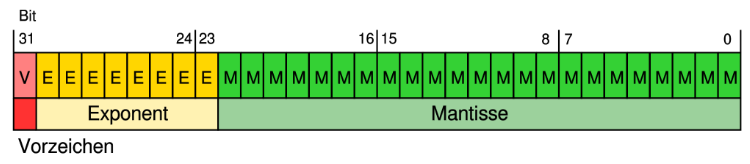
\includegraphics[width=\linewidth]{pics/floatingpoint}
	\caption{32bit Fließkomma (single)}
\end{figure}

\subsubsection*{Standartgrößen}
\begin{itemize}

	\item Single: 32Bit \\
	VZ = 1Bit, EXP = 8Bit, MAN = 23Bit, B = 127
	
	\item Double: 64Bit \\
	VZ = 1Bit, EXP = 11Bit, MAN = 52Bit, B = 1023

\end{itemize}

\subsubsection*{Berechnung}
\begin{itemize}

	\item Dezimal zu Binär \\
	Für die Dezimalzahl \textbf{x} wiederhole:
	\begin{itemize}
		\item $\widetilde{x} := 2 \cdot x$
		\item $b_i = \widetilde{x}\text{ div }1$
		\item $x := \widetilde{x}\text{ mod }1$
	\end{itemize}
	Ergebnis: $0.b_1b_2...b_n$
	
	\item Normalisierung $M = (0:=+, 1:=-) 1.m \cdot 2^E$ \\
	
	\item Exponent $e = E - B$ \\

\end{itemize}

\subsubsection*{Rundungsfehler}
\begin{itemize}

	\item Auslöschung \\
	Subtraktion gleichgroßer Zahlen $\Rightarrow$ Ergebnis wird durch 0ller aufgefüllt
	
	\item Angleichung \\
	Addition oder Subtraktion, betragsmäßig sehr unterschiedlicher Zahlen

\end{itemize}

\subsection{Formeln}
\begin{itemize}

	\item Absoluter Fehler: $\bigtriangleup x = |x - \widetilde{x}|$
	
	\item Relativer Fehler: $rel = \frac{\bigtriangleup x}{|x|}$
	
	\item Maschinengenauigkeit: $\epsilon = 2^{-n}$
	
	\item Kondition (Verstärkung von Eingabefehlern zu Ausgabefehlern) \\
	$\kappa = \bigg|\frac{f'(x)}{f(x)} \cdot x\bigg|$\\
	(schlechte Kondition wenn $\kappa \gg 1$)
	
	\item Taylorreihen
	\begin{itemize}
		\item $sin(x) = x - \frac{x^3}{6} + \frac{x^5}{120} - \cdots$
		\item $cos(x) = 1 - \frac{x^2}{2} + \frac{x^4}{24} - \frac{x^6}{720} + \cdots$
		\item $e^x = 1 + x + \frac{x^2}{2} + \frac{x^3}{6} + \frac{x^4}{24} + \frac{x^5}{120} + \frac{x^6}{720}$
	\end{itemize}
	
	\item Trigonometrische Umformungen
	\begin{itemize}
		\item $sin(\alpha )^2 + cos(\alpha )^2 = 1$
		\item $sin(-\alpha ) = -sin(\alpha )$
		\item $cos(-\alpha ) = cos(\alpha )$
		\item $sin(2 \alpha ) = 2 sin(\alpha ) cos(\alpha )$
		\item $cos(2 \alpha ) = cos(\alpha )^2 - sin(\alpha )^2$
		\item $sin(\alpha + \beta ) = cos(\alpha ) sin(\beta ) - sin(\alpha ) cos(\beta )$
	\end{itemize}
	
	\item Ableitung von Grundfunktionen
	\begin{itemize}
		\item $(sin(x))' = cos(x)$
		\item $(cos(x))' = -sin(x)$
		\item $(ln(x))' = \frac{1}{x}$
	\end{itemize}

\end{itemize}
